\section{Preliminary Data Exploration}
% \begin{itemize}
%     \item Which features are in your dataset?
%     \item How are your features distributed?
%     \item Are some of your features correlated with each other or with the target label?
%     \item How many classes are there and are they balanced?
%     \item Does some of the information here contradict or confirm prior domain knowledge?
%     \item Are there any missing values, or outliers in your data?
%     \item Which plots will you include to show what your dataset is all about?
%     \item Don't forget to interpret your plots.
%     \item \textbf{Required:} 1 dimensionality reduced plot, 2 other plots.
% \end{itemize}

The dataset we found on GitHub contains 3-axis gyroscope readings (GYR) and 3-axis accelerometer readings (ACC) over time, where Figure \ref{fig:axes} shows the sensor axes. Figure \ref{fig:raw_signals} shows an example signal. This gives us the channels ACC$_x$, ACC$_y$, ACC$_z$, GYR$_x$, GYR$_y$, and GYR$_z$, each sampled at 50 Hz. As an exploration, we applied a low-pass filter to the raw signals to reduce noise, as shown in Figure \ref{fig:smoothed_signals}. Since the task we are framing is a binary verification problem, the class balance can be controlled during training by pairing each positive example with a negative comparison example.

\begin{figure}[H]
    \centering
    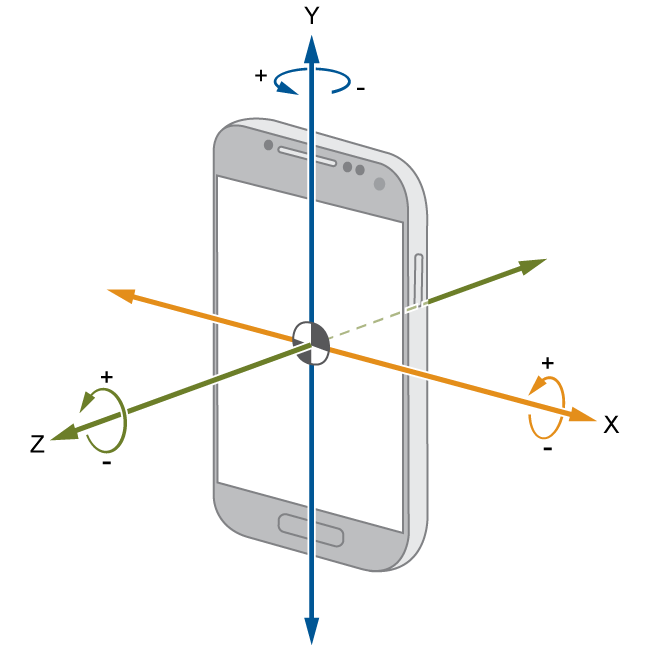
\includegraphics[width=0.5\textwidth]{figures/axes.png}
    \caption{Sensor axes for accelerometer and gyroscope readings \cite{mathworks2014gyroscope}}
    \label{fig:axes}
\end{figure}

\begin{figure}[H]
    \centering
    \begin{subfigure}[t]{0.48\textwidth}
        \centering
        
\includegraphics[width=\textwidth]{figures/raw_signals.png}
        \caption{Raw Sensor Signals Over Time}
        \label{fig:raw_signals}
    \end{subfigure}\hfill
    \begin{subfigure}[t]{0.48\textwidth}
        \centering
        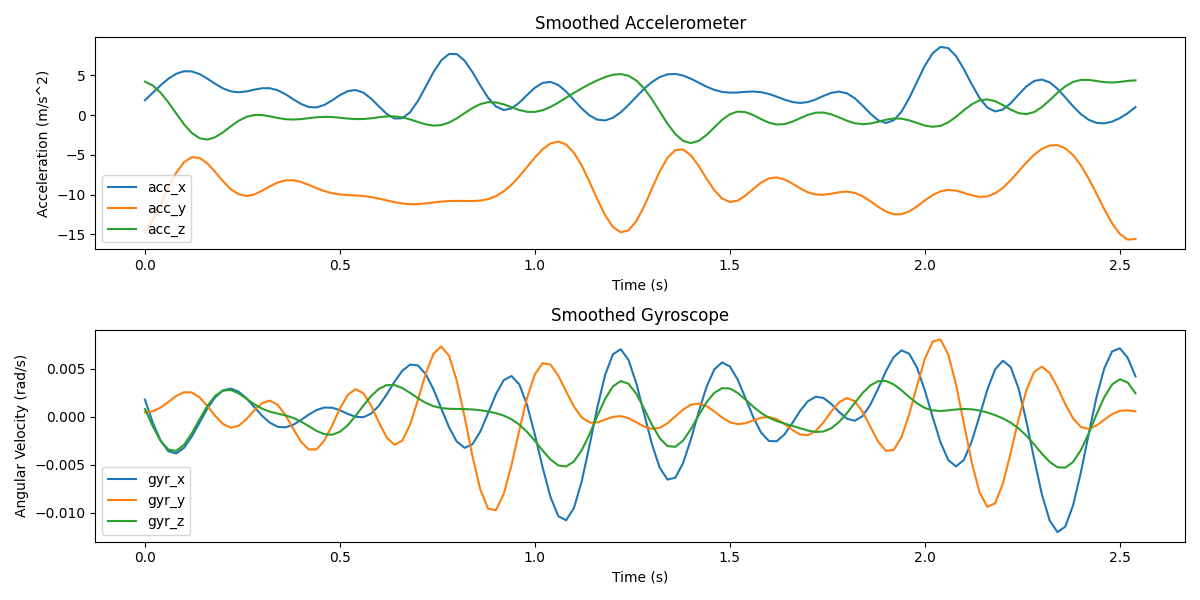
\includegraphics[width=\textwidth]{figures/smoothed_signals.png}
        \caption{Smoothed Sensor Signals Over Time}
        \label{fig:smoothed_signals}
    \end{subfigure}
    \caption{Time-series sensor signal examples}
    \label{fig:signal_examples}
\end{figure}

% There is naturally correlation in the data because these channels represent different axes in the same physical space, but this is not necessarily a limitation. Instead, the channels are complementary because together they capture spatial information about the motion of a step and its effect on acceleration and rotation. This generally supports our original expectations rather than contradicting them.

We also computed the correlation matrix of the six sensor channels, which is shown in Figure \ref{fig:correlation}. Even though majority of absolute value of channel correlations are close to zero (< 0.1), there can be seen a slight positive correlation of 0.355 between GYR$_x$ and ACC$_z$. They are predicted to be correlated because both channels are influenced by the inward motion of the leg during walking, where GYR$_x$ captures the femur rotation and ACC$_z$ captures the vertical acceleration from leg lifting.

Accompanying it, there is a negative correlation of -0.229 between GYR$_z$ and ACC$_x$, which can be explained by the swinging motion of the leg during walking. 

\begin{figure}[H]
    \centering
    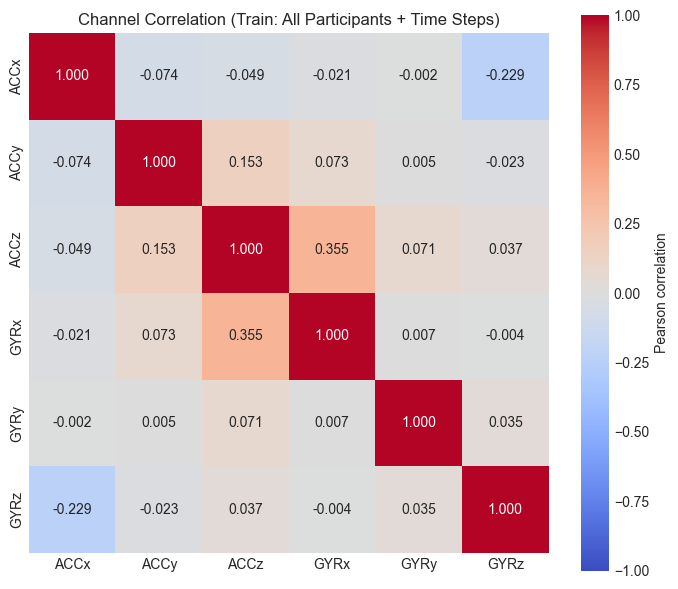
\includegraphics[width=0.7\textwidth]{figures/correlation.png}
    \caption{Correlation Matrix of Sensor Readings}
    \label{fig:correlation}
\end{figure}
